% Created by tikzDevice version 0.12.6 on 2025-02-06 14:05:59
% !TEX encoding = UTF-8 Unicode
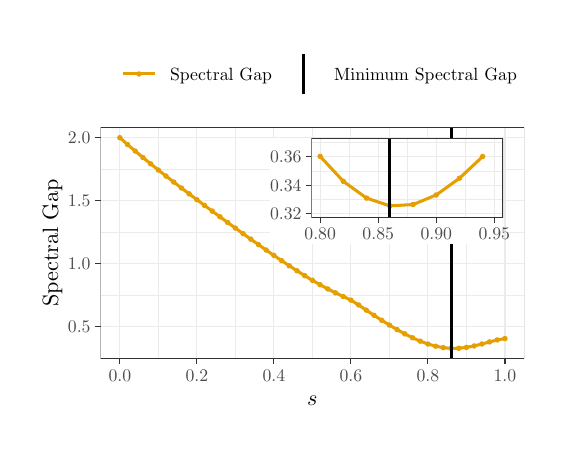
\begin{tikzpicture}[x=1pt,y=1pt]
\definecolor{fillColor}{RGB}{255,255,255}
\path[use as bounding box,fill=fillColor,fill opacity=0.00] (0,0) rectangle (184.92,143.50);
\begin{scope}
\path[clip] (  0.00,  0.00) rectangle (184.92,143.50);
\definecolor{drawColor}{RGB}{255,255,255}
\definecolor{fillColor}{RGB}{255,255,255}

\path[draw=drawColor,line width= 0.6pt,line join=round,line cap=round,fill=fillColor] (  0.00,  0.00) rectangle (184.92,143.50);
\end{scope}
\begin{scope}
\path[clip] (  5.50,  5.50) rectangle (179.42,138.00);
\definecolor{drawColor}{RGB}{255,255,255}
\definecolor{fillColor}{RGB}{255,255,255}

\path[draw=drawColor,line width= 0.4pt,line join=round,line cap=round,fill=fillColor] (  5.50,  5.50) rectangle (179.42,138.00);
\end{scope}
\begin{scope}
\path[clip] ( 26.34, 23.82) rectangle (179.42,107.55);
\definecolor{fillColor}{RGB}{255,255,255}

\path[fill=fillColor] ( 26.34, 23.82) rectangle (179.42,107.55);
\definecolor{drawColor}{gray}{0.92}

\path[draw=drawColor,line width= 0.2pt,line join=round] ( 26.34, 24.19) --
	(179.42, 24.19);

\path[draw=drawColor,line width= 0.2pt,line join=round] ( 26.34, 46.92) --
	(179.42, 46.92);

\path[draw=drawColor,line width= 0.2pt,line join=round] ( 26.34, 69.65) --
	(179.42, 69.65);

\path[draw=drawColor,line width= 0.2pt,line join=round] ( 26.34, 92.37) --
	(179.42, 92.37);

\path[draw=drawColor,line width= 0.2pt,line join=round] ( 47.21, 23.82) --
	( 47.21,107.55);

\path[draw=drawColor,line width= 0.2pt,line join=round] ( 75.05, 23.82) --
	( 75.05,107.55);

\path[draw=drawColor,line width= 0.2pt,line join=round] (102.88, 23.82) --
	(102.88,107.55);

\path[draw=drawColor,line width= 0.2pt,line join=round] (130.71, 23.82) --
	(130.71,107.55);

\path[draw=drawColor,line width= 0.2pt,line join=round] (158.54, 23.82) --
	(158.54,107.55);

\path[draw=drawColor,line width= 0.4pt,line join=round] ( 26.34, 35.55) --
	(179.42, 35.55);

\path[draw=drawColor,line width= 0.4pt,line join=round] ( 26.34, 58.28) --
	(179.42, 58.28);

\path[draw=drawColor,line width= 0.4pt,line join=round] ( 26.34, 81.01) --
	(179.42, 81.01);

\path[draw=drawColor,line width= 0.4pt,line join=round] ( 26.34,103.74) --
	(179.42,103.74);

\path[draw=drawColor,line width= 0.4pt,line join=round] ( 33.30, 23.82) --
	( 33.30,107.55);

\path[draw=drawColor,line width= 0.4pt,line join=round] ( 61.13, 23.82) --
	( 61.13,107.55);

\path[draw=drawColor,line width= 0.4pt,line join=round] ( 88.96, 23.82) --
	( 88.96,107.55);

\path[draw=drawColor,line width= 0.4pt,line join=round] (116.79, 23.82) --
	(116.79,107.55);

\path[draw=drawColor,line width= 0.4pt,line join=round] (144.63, 23.82) --
	(144.63,107.55);

\path[draw=drawColor,line width= 0.4pt,line join=round] (172.46, 23.82) --
	(172.46,107.55);
\definecolor{drawColor}{RGB}{230,159,0}

\path[draw=drawColor,line width= 1.1pt,line join=round] ( 33.30,103.74) --
	( 36.08,101.28) --
	( 38.87, 98.91) --
	( 41.65, 96.58) --
	( 44.43, 94.31) --
	( 47.21, 92.07) --
	( 50.00, 89.87) --
	( 52.78, 87.71) --
	( 55.56, 85.57) --
	( 58.35, 83.45) --
	( 61.13, 81.36) --
	( 63.91, 79.27) --
	( 66.70, 77.21) --
	( 69.48, 75.15) --
	( 72.26, 73.11) --
	( 75.05, 71.09) --
	( 77.83, 69.07) --
	( 80.61, 67.08) --
	( 83.40, 65.10) --
	( 86.18, 63.14) --
	( 88.96, 61.21) --
	( 91.75, 59.32) --
	( 94.53, 57.46) --
	( 97.31, 55.65) --
	(100.10, 53.89) --
	(102.88, 52.20) --
	(105.66, 50.60) --
	(108.45, 49.09) --
	(111.23, 47.68) --
	(114.01, 46.37) --
	(116.79, 45.05) --
	(119.58, 43.30) --
	(122.36, 41.42) --
	(125.14, 39.57) --
	(127.93, 37.77) --
	(130.71, 36.04) --
	(133.49, 34.39) --
	(136.28, 32.86) --
	(139.06, 31.45) --
	(141.84, 30.22) --
	(144.63, 29.20) --
	(147.41, 28.40) --
	(150.19, 27.87) --
	(152.98, 27.62) --
	(155.76, 27.66) --
	(158.54, 27.97) --
	(161.33, 28.50) --
	(164.11, 29.19) --
	(166.89, 29.95) --
	(169.68, 30.66) --
	(172.46, 31.16);
\definecolor{fillColor}{RGB}{230,159,0}

\path[draw=drawColor,line width= 0.4pt,line join=round,line cap=round,fill=fillColor] ( 33.30,103.74) circle (  0.78);

\path[draw=drawColor,line width= 0.4pt,line join=round,line cap=round,fill=fillColor] ( 36.08,101.28) circle (  0.78);

\path[draw=drawColor,line width= 0.4pt,line join=round,line cap=round,fill=fillColor] ( 38.87, 98.91) circle (  0.78);

\path[draw=drawColor,line width= 0.4pt,line join=round,line cap=round,fill=fillColor] ( 41.65, 96.58) circle (  0.78);

\path[draw=drawColor,line width= 0.4pt,line join=round,line cap=round,fill=fillColor] ( 44.43, 94.31) circle (  0.78);

\path[draw=drawColor,line width= 0.4pt,line join=round,line cap=round,fill=fillColor] ( 47.21, 92.07) circle (  0.78);

\path[draw=drawColor,line width= 0.4pt,line join=round,line cap=round,fill=fillColor] ( 50.00, 89.87) circle (  0.78);

\path[draw=drawColor,line width= 0.4pt,line join=round,line cap=round,fill=fillColor] ( 52.78, 87.71) circle (  0.78);

\path[draw=drawColor,line width= 0.4pt,line join=round,line cap=round,fill=fillColor] ( 55.56, 85.57) circle (  0.78);

\path[draw=drawColor,line width= 0.4pt,line join=round,line cap=round,fill=fillColor] ( 58.35, 83.45) circle (  0.78);

\path[draw=drawColor,line width= 0.4pt,line join=round,line cap=round,fill=fillColor] ( 61.13, 81.36) circle (  0.78);

\path[draw=drawColor,line width= 0.4pt,line join=round,line cap=round,fill=fillColor] ( 63.91, 79.27) circle (  0.78);

\path[draw=drawColor,line width= 0.4pt,line join=round,line cap=round,fill=fillColor] ( 66.70, 77.21) circle (  0.78);

\path[draw=drawColor,line width= 0.4pt,line join=round,line cap=round,fill=fillColor] ( 69.48, 75.15) circle (  0.78);

\path[draw=drawColor,line width= 0.4pt,line join=round,line cap=round,fill=fillColor] ( 72.26, 73.11) circle (  0.78);

\path[draw=drawColor,line width= 0.4pt,line join=round,line cap=round,fill=fillColor] ( 75.05, 71.09) circle (  0.78);

\path[draw=drawColor,line width= 0.4pt,line join=round,line cap=round,fill=fillColor] ( 77.83, 69.07) circle (  0.78);

\path[draw=drawColor,line width= 0.4pt,line join=round,line cap=round,fill=fillColor] ( 80.61, 67.08) circle (  0.78);

\path[draw=drawColor,line width= 0.4pt,line join=round,line cap=round,fill=fillColor] ( 83.40, 65.10) circle (  0.78);

\path[draw=drawColor,line width= 0.4pt,line join=round,line cap=round,fill=fillColor] ( 86.18, 63.14) circle (  0.78);

\path[draw=drawColor,line width= 0.4pt,line join=round,line cap=round,fill=fillColor] ( 88.96, 61.21) circle (  0.78);

\path[draw=drawColor,line width= 0.4pt,line join=round,line cap=round,fill=fillColor] ( 91.75, 59.32) circle (  0.78);

\path[draw=drawColor,line width= 0.4pt,line join=round,line cap=round,fill=fillColor] ( 94.53, 57.46) circle (  0.78);

\path[draw=drawColor,line width= 0.4pt,line join=round,line cap=round,fill=fillColor] ( 97.31, 55.65) circle (  0.78);

\path[draw=drawColor,line width= 0.4pt,line join=round,line cap=round,fill=fillColor] (100.10, 53.89) circle (  0.78);

\path[draw=drawColor,line width= 0.4pt,line join=round,line cap=round,fill=fillColor] (102.88, 52.20) circle (  0.78);

\path[draw=drawColor,line width= 0.4pt,line join=round,line cap=round,fill=fillColor] (105.66, 50.60) circle (  0.78);

\path[draw=drawColor,line width= 0.4pt,line join=round,line cap=round,fill=fillColor] (108.45, 49.09) circle (  0.78);

\path[draw=drawColor,line width= 0.4pt,line join=round,line cap=round,fill=fillColor] (111.23, 47.68) circle (  0.78);

\path[draw=drawColor,line width= 0.4pt,line join=round,line cap=round,fill=fillColor] (114.01, 46.37) circle (  0.78);

\path[draw=drawColor,line width= 0.4pt,line join=round,line cap=round,fill=fillColor] (116.79, 45.05) circle (  0.78);

\path[draw=drawColor,line width= 0.4pt,line join=round,line cap=round,fill=fillColor] (119.58, 43.30) circle (  0.78);

\path[draw=drawColor,line width= 0.4pt,line join=round,line cap=round,fill=fillColor] (122.36, 41.42) circle (  0.78);

\path[draw=drawColor,line width= 0.4pt,line join=round,line cap=round,fill=fillColor] (125.14, 39.57) circle (  0.78);

\path[draw=drawColor,line width= 0.4pt,line join=round,line cap=round,fill=fillColor] (127.93, 37.77) circle (  0.78);

\path[draw=drawColor,line width= 0.4pt,line join=round,line cap=round,fill=fillColor] (130.71, 36.04) circle (  0.78);

\path[draw=drawColor,line width= 0.4pt,line join=round,line cap=round,fill=fillColor] (133.49, 34.39) circle (  0.78);

\path[draw=drawColor,line width= 0.4pt,line join=round,line cap=round,fill=fillColor] (136.28, 32.86) circle (  0.78);

\path[draw=drawColor,line width= 0.4pt,line join=round,line cap=round,fill=fillColor] (139.06, 31.45) circle (  0.78);

\path[draw=drawColor,line width= 0.4pt,line join=round,line cap=round,fill=fillColor] (141.84, 30.22) circle (  0.78);

\path[draw=drawColor,line width= 0.4pt,line join=round,line cap=round,fill=fillColor] (144.63, 29.20) circle (  0.78);

\path[draw=drawColor,line width= 0.4pt,line join=round,line cap=round,fill=fillColor] (147.41, 28.40) circle (  0.78);

\path[draw=drawColor,line width= 0.4pt,line join=round,line cap=round,fill=fillColor] (150.19, 27.87) circle (  0.78);

\path[draw=drawColor,line width= 0.4pt,line join=round,line cap=round,fill=fillColor] (152.98, 27.62) circle (  0.78);

\path[draw=drawColor,line width= 0.4pt,line join=round,line cap=round,fill=fillColor] (155.76, 27.66) circle (  0.78);

\path[draw=drawColor,line width= 0.4pt,line join=round,line cap=round,fill=fillColor] (158.54, 27.97) circle (  0.78);

\path[draw=drawColor,line width= 0.4pt,line join=round,line cap=round,fill=fillColor] (161.33, 28.50) circle (  0.78);

\path[draw=drawColor,line width= 0.4pt,line join=round,line cap=round,fill=fillColor] (164.11, 29.19) circle (  0.78);

\path[draw=drawColor,line width= 0.4pt,line join=round,line cap=round,fill=fillColor] (166.89, 29.95) circle (  0.78);

\path[draw=drawColor,line width= 0.4pt,line join=round,line cap=round,fill=fillColor] (169.68, 30.66) circle (  0.78);

\path[draw=drawColor,line width= 0.4pt,line join=round,line cap=round,fill=fillColor] (172.46, 31.16) circle (  0.78);
\definecolor{drawColor}{RGB}{0,0,0}

\path[draw=drawColor,line width= 1.1pt,line join=round] (152.98, 23.82) -- (152.98,107.55);
\definecolor{drawColor}{gray}{0.20}

\path[draw=drawColor,line width= 0.4pt,line join=round,line cap=round] ( 26.34, 23.82) rectangle (179.42,107.55);
\end{scope}
\begin{scope}
\path[clip] (  0.00,  0.00) rectangle (184.92,143.50);
\definecolor{drawColor}{gray}{0.30}

\node[text=drawColor,anchor=base east,inner sep=0pt, outer sep=0pt, scale=  0.64] at ( 22.74, 33.35) {0.5};

\node[text=drawColor,anchor=base east,inner sep=0pt, outer sep=0pt, scale=  0.64] at ( 22.74, 56.08) {1.0};

\node[text=drawColor,anchor=base east,inner sep=0pt, outer sep=0pt, scale=  0.64] at ( 22.74, 78.81) {1.5};

\node[text=drawColor,anchor=base east,inner sep=0pt, outer sep=0pt, scale=  0.64] at ( 22.74,101.54) {2.0};
\end{scope}
\begin{scope}
\path[clip] (  0.00,  0.00) rectangle (184.92,143.50);
\definecolor{drawColor}{gray}{0.20}

\path[draw=drawColor,line width= 0.4pt,line join=round] ( 24.34, 35.55) --
	( 26.34, 35.55);

\path[draw=drawColor,line width= 0.4pt,line join=round] ( 24.34, 58.28) --
	( 26.34, 58.28);

\path[draw=drawColor,line width= 0.4pt,line join=round] ( 24.34, 81.01) --
	( 26.34, 81.01);

\path[draw=drawColor,line width= 0.4pt,line join=round] ( 24.34,103.74) --
	( 26.34,103.74);
\end{scope}
\begin{scope}
\path[clip] (  0.00,  0.00) rectangle (184.92,143.50);
\definecolor{drawColor}{gray}{0.20}

\path[draw=drawColor,line width= 0.4pt,line join=round] ( 33.30, 21.82) --
	( 33.30, 23.82);

\path[draw=drawColor,line width= 0.4pt,line join=round] ( 61.13, 21.82) --
	( 61.13, 23.82);

\path[draw=drawColor,line width= 0.4pt,line join=round] ( 88.96, 21.82) --
	( 88.96, 23.82);

\path[draw=drawColor,line width= 0.4pt,line join=round] (116.79, 21.82) --
	(116.79, 23.82);

\path[draw=drawColor,line width= 0.4pt,line join=round] (144.63, 21.82) --
	(144.63, 23.82);

\path[draw=drawColor,line width= 0.4pt,line join=round] (172.46, 21.82) --
	(172.46, 23.82);
\end{scope}
\begin{scope}
\path[clip] (  0.00,  0.00) rectangle (184.92,143.50);
\definecolor{drawColor}{gray}{0.30}

\node[text=drawColor,anchor=base,inner sep=0pt, outer sep=0pt, scale=  0.64] at ( 33.30, 15.81) {0.0};

\node[text=drawColor,anchor=base,inner sep=0pt, outer sep=0pt, scale=  0.64] at ( 61.13, 15.81) {0.2};

\node[text=drawColor,anchor=base,inner sep=0pt, outer sep=0pt, scale=  0.64] at ( 88.96, 15.81) {0.4};

\node[text=drawColor,anchor=base,inner sep=0pt, outer sep=0pt, scale=  0.64] at (116.79, 15.81) {0.6};

\node[text=drawColor,anchor=base,inner sep=0pt, outer sep=0pt, scale=  0.64] at (144.63, 15.81) {0.8};

\node[text=drawColor,anchor=base,inner sep=0pt, outer sep=0pt, scale=  0.64] at (172.46, 15.81) {1.0};
\end{scope}
\begin{scope}
\path[clip] (  0.00,  0.00) rectangle (184.92,143.50);
\definecolor{drawColor}{RGB}{0,0,0}

\node[text=drawColor,anchor=base,inner sep=0pt, outer sep=0pt, scale=  0.80] at (102.88,  7.06) {$s$};
\end{scope}
\begin{scope}
\path[clip] (  0.00,  0.00) rectangle (184.92,143.50);
\definecolor{drawColor}{RGB}{0,0,0}

\node[text=drawColor,rotate= 90.00,anchor=base,inner sep=0pt, outer sep=0pt, scale=  0.80] at ( 11.01, 65.68) {Spectral Gap};
\end{scope}
\begin{scope}
\path[clip] (  0.00,  0.00) rectangle (184.92,143.50);
\definecolor{fillColor}{RGB}{255,255,255}

\path[fill=fillColor] ( 25.00,115.55) rectangle (180.76,138.00);
\end{scope}
\begin{scope}
\path[clip] (  0.00,  0.00) rectangle (184.92,143.50);
\definecolor{fillColor}{RGB}{255,255,255}

\path[fill=fillColor] ( 33.00,119.55) rectangle ( 47.45,134.00);
\end{scope}
\begin{scope}
\path[clip] (  0.00,  0.00) rectangle (184.92,143.50);
\definecolor{drawColor}{RGB}{230,159,0}

\path[draw=drawColor,line width= 1.1pt,line join=round] ( 34.44,126.77) -- ( 46.01,126.77);
\end{scope}
\begin{scope}
\path[clip] (  0.00,  0.00) rectangle (184.92,143.50);
\definecolor{drawColor}{RGB}{230,159,0}
\definecolor{fillColor}{RGB}{230,159,0}

\path[draw=drawColor,line width= 0.4pt,line join=round,line cap=round,fill=fillColor] ( 40.22,126.77) circle (  0.78);
\end{scope}
\begin{scope}
\path[clip] (  0.00,  0.00) rectangle (184.92,143.50);
\definecolor{fillColor}{RGB}{255,255,255}

\path[fill=fillColor] ( 92.30,119.55) rectangle (106.76,134.00);
\end{scope}
\begin{scope}
\path[clip] (  0.00,  0.00) rectangle (184.92,143.50);
\definecolor{drawColor}{RGB}{0,0,0}

\path[draw=drawColor,line width= 1.1pt,line join=round] ( 99.53,119.55) -- ( 99.53,134.00);
\end{scope}
\begin{scope}
\path[clip] (  0.00,  0.00) rectangle (184.92,143.50);
\definecolor{drawColor}{RGB}{0,0,0}

\node[text=drawColor,anchor=base west,inner sep=0pt, outer sep=0pt, scale=  0.64] at ( 51.45,124.57) {Spectral Gap};
\end{scope}
\begin{scope}
\path[clip] (  0.00,  0.00) rectangle (184.92,143.50);
\definecolor{drawColor}{RGB}{0,0,0}

\node[text=drawColor,anchor=base west,inner sep=0pt, outer sep=0pt, scale=  0.64] at (110.76,124.57) {Minimum Spectral Gap};
\end{scope}
\begin{scope}
\path[clip] ( 87.57, 65.68) rectangle (171.76,103.36);
\definecolor{drawColor}{RGB}{255,255,255}
\definecolor{fillColor}{RGB}{255,255,255}

\path[draw=drawColor,line width= 0.4pt,line join=round,line cap=round,fill=fillColor] ( 87.57, 65.68) rectangle (171.76,103.36);
\end{scope}
\begin{scope}
\path[clip] (102.55, 74.93) rectangle (171.76,103.36);
\definecolor{fillColor}{RGB}{255,255,255}

\path[fill=fillColor] (102.55, 74.93) rectangle (171.76,103.36);
\definecolor{drawColor}{gray}{0.92}

\path[draw=drawColor,line width= 0.2pt,line join=round] (102.55, 81.39) --
	(171.76, 81.39);

\path[draw=drawColor,line width= 0.2pt,line join=round] (102.55, 91.73) --
	(171.76, 91.73);

\path[draw=drawColor,line width= 0.2pt,line join=round] (102.55,102.07) --
	(171.76,102.07);

\path[draw=drawColor,line width= 0.2pt,line join=round] (116.18, 74.93) --
	(116.18,103.36);

\path[draw=drawColor,line width= 0.2pt,line join=round] (137.15, 74.93) --
	(137.15,103.36);

\path[draw=drawColor,line width= 0.2pt,line join=round] (158.13, 74.93) --
	(158.13,103.36);

\path[draw=drawColor,line width= 0.4pt,line join=round] (102.55, 76.23) --
	(171.76, 76.23);

\path[draw=drawColor,line width= 0.4pt,line join=round] (102.55, 86.56) --
	(171.76, 86.56);

\path[draw=drawColor,line width= 0.4pt,line join=round] (102.55, 96.90) --
	(171.76, 96.90);

\path[draw=drawColor,line width= 0.4pt,line join=round] (105.69, 74.93) --
	(105.69,103.36);

\path[draw=drawColor,line width= 0.4pt,line join=round] (126.67, 74.93) --
	(126.67,103.36);

\path[draw=drawColor,line width= 0.4pt,line join=round] (147.64, 74.93) --
	(147.64,103.36);

\path[draw=drawColor,line width= 0.4pt,line join=round] (168.62, 74.93) --
	(168.62,103.36);
\definecolor{drawColor}{RGB}{230,159,0}

\path[draw=drawColor,line width= 1.1pt,line join=round] (105.69, 97.00) --
	(114.08, 87.96) --
	(122.47, 81.91) --
	(130.86, 79.12) --
	(139.25, 79.58) --
	(147.64, 83.05) --
	(156.03, 89.09) --
	(164.42, 96.95);
\definecolor{fillColor}{RGB}{230,159,0}

\path[draw=drawColor,line width= 0.4pt,line join=round,line cap=round,fill=fillColor] (105.69, 97.00) circle (  0.78);

\path[draw=drawColor,line width= 0.4pt,line join=round,line cap=round,fill=fillColor] (114.08, 87.96) circle (  0.78);

\path[draw=drawColor,line width= 0.4pt,line join=round,line cap=round,fill=fillColor] (122.47, 81.91) circle (  0.78);

\path[draw=drawColor,line width= 0.4pt,line join=round,line cap=round,fill=fillColor] (130.86, 79.12) circle (  0.78);

\path[draw=drawColor,line width= 0.4pt,line join=round,line cap=round,fill=fillColor] (139.25, 79.58) circle (  0.78);

\path[draw=drawColor,line width= 0.4pt,line join=round,line cap=round,fill=fillColor] (147.64, 83.05) circle (  0.78);

\path[draw=drawColor,line width= 0.4pt,line join=round,line cap=round,fill=fillColor] (156.03, 89.09) circle (  0.78);

\path[draw=drawColor,line width= 0.4pt,line join=round,line cap=round,fill=fillColor] (164.42, 96.95) circle (  0.78);
\definecolor{drawColor}{RGB}{0,0,0}

\path[draw=drawColor,line width= 1.1pt,line join=round] (130.86, 74.93) -- (130.86,103.36);
\definecolor{drawColor}{gray}{0.20}

\path[draw=drawColor,line width= 0.4pt,line join=round,line cap=round] (102.55, 74.93) rectangle (171.76,103.36);
\end{scope}
\begin{scope}
\path[clip] (  0.00,  0.00) rectangle (184.92,143.50);
\definecolor{drawColor}{gray}{0.30}

\node[text=drawColor,anchor=base east,inner sep=0pt, outer sep=0pt, scale=  0.64] at ( 98.95, 74.02) {0.32};

\node[text=drawColor,anchor=base east,inner sep=0pt, outer sep=0pt, scale=  0.64] at ( 98.95, 84.36) {0.34};

\node[text=drawColor,anchor=base east,inner sep=0pt, outer sep=0pt, scale=  0.64] at ( 98.95, 94.69) {0.36};
\end{scope}
\begin{scope}
\path[clip] (  0.00,  0.00) rectangle (184.92,143.50);
\definecolor{drawColor}{gray}{0.20}

\path[draw=drawColor,line width= 0.4pt,line join=round] (100.55, 76.23) --
	(102.55, 76.23);

\path[draw=drawColor,line width= 0.4pt,line join=round] (100.55, 86.56) --
	(102.55, 86.56);

\path[draw=drawColor,line width= 0.4pt,line join=round] (100.55, 96.90) --
	(102.55, 96.90);
\end{scope}
\begin{scope}
\path[clip] (  0.00,  0.00) rectangle (184.92,143.50);
\definecolor{drawColor}{gray}{0.20}

\path[draw=drawColor,line width= 0.4pt,line join=round] (105.69, 72.93) --
	(105.69, 74.93);

\path[draw=drawColor,line width= 0.4pt,line join=round] (126.67, 72.93) --
	(126.67, 74.93);

\path[draw=drawColor,line width= 0.4pt,line join=round] (147.64, 72.93) --
	(147.64, 74.93);

\path[draw=drawColor,line width= 0.4pt,line join=round] (168.62, 72.93) --
	(168.62, 74.93);
\end{scope}
\begin{scope}
\path[clip] (  0.00,  0.00) rectangle (184.92,143.50);
\definecolor{drawColor}{gray}{0.30}

\node[text=drawColor,anchor=base,inner sep=0pt, outer sep=0pt, scale=  0.64] at (105.69, 66.93) {0.80};

\node[text=drawColor,anchor=base,inner sep=0pt, outer sep=0pt, scale=  0.64] at (126.67, 66.93) {0.85};

\node[text=drawColor,anchor=base,inner sep=0pt, outer sep=0pt, scale=  0.64] at (147.64, 66.93) {0.90};

\node[text=drawColor,anchor=base,inner sep=0pt, outer sep=0pt, scale=  0.64] at (168.62, 66.93) {0.95};
\end{scope}
\end{tikzpicture}
